\documentclass[tikz,border=10pt]{standalone}

\usepackage{tikz}
\usepackage{amssymb,amsmath,amsthm,amsfonts}

\newcommand{\ket}[1]{\left| #1 \right \rangle}

\begin{document}


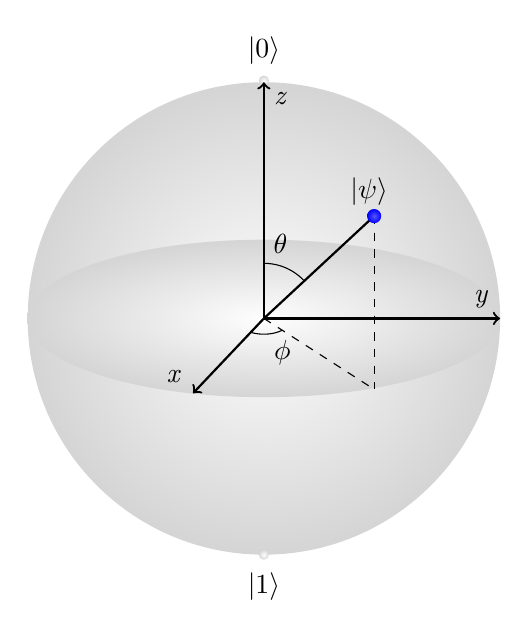
\begin{tikzpicture}

\draw[dashed] (3,3) -- (3,0);

\shade[inner color={rgb:black,1;white,200} ,outer color={rgb:black,1;white,5}  ] (3,3) circle (3cm);
\shade[inner color={rgb:black,1;white,200} ,outer color={rgb:black,1;white,5}  ]  (3,3) ellipse (3cm and 1cm);

\shade[inner color={rgb:black,1;white,200} ,outer color={rgb:black,1;white,5}  ]  (3,6.02) circle (0.065cm);

\draw (3,6.1) node[anchor=south] {\textit{$ \ket{0}$}} ;
\draw (3,-0.1) node[anchor=north] {\textit{$ \ket{1}$}} ;

\draw[thick,->] (3,3) -- (3,6)  node[anchor=north west] {\textit{z}} ;
\draw[thick,->] (3,3) -- (6,3) node[anchor= south east] {\textit{y}} ;
\draw[thick,->] (3,3) -- (2.1,2.05) node[anchor= south east] {\textit{x}} ;

\draw[thick] (3,3) -- (4.4,4.3)  node[anchor= south] {\textit{$ \ket{\psi}$ } } ;

\draw [domain=43.8:90] plot ({3 + 0.7*cos(\x)}, {3 + 0.7*sin(\x)}) node[anchor= south west]  {\textit{$\theta$}};
\draw [domain=240:312] plot ({3 + 0.35*cos(\x)}, {3 + 0.2*sin(\x)}) node[anchor= north]  {\textit{$\phi$}};
 
\draw[dashed] (4.4,4.3) -- (4.4,2.1) ;
\draw[dashed] (4.4,4.3) -- (4.4,2.1) ;
\draw[dashed] (3,3) -- (4.4,2.1) ;

\shade[inner color={rgb:blue,2;white,1} ,outer color={rgb:blue,3}  ] (4.4,4.3) circle (0.09cm);

\shade[inner color={rgb:black,1;white,200} ,outer color={rgb:black,1;white,5}  ]   (3,0) circle (0.065cm);

\end{tikzpicture}


\end{document}